%\documentclass[a4paper]{article}
%\usepackage[T1]{fontenc}
%\usepackage[utf8]{inputenc}
%\usepackage[italian]{babel}
%\usepackage{amssymb}
%\usepackage{amsmath}
%\usepackage{hyperref}
%\usepackage{amsthm}
%\usepackage{graphicx}
\documentclass[journal, a4paper]{IEEEtran}
\usepackage[italian]{babel}
\usepackage{booktabs}
\usepackage{siunitx}%Questo serve a caricare il pacchetto delle unità di misura del sistema internazionale%
\usepackage[utf8]{inputenc}
\usepackage{graphicx} 
\usepackage{url}
\usepackage{amsmath}


\usepackage{keyval}
\usepackage{xcolor}
\usepackage{caption}
\usepackage{tikz}
\usepackage{circuitikz}
\usepackage{authblk}
%\usepackage{hyperref}

\begin{document}


% Define document title and author
	\title{Tecnologie Digitali - Logbook Week 1}
	\author[1]{Salvatore Bottaro}
		\author[2]{Lorenzo M. Perrone}
		\affil[1]{\texttt{email@sa.com}}
		\affil[2]{\texttt{lorenzo.perrone.lmp@gmail.com}}
	\markboth{Tecnologie Digitali - Di Lieto}{}
	\maketitle
	
\begin{abstract}
	Logbook di laboratorio di Tecnologie Digitali, a.a. 2015/2016. Week 1.
\end{abstract}

\section{Lezione 28/09/2015}
Abbiamo misurato la d.d.p. $V_{out}$ ai capi della resistenza $R_2$ di un partitore di tensione secondo il seguente schema circuitale:\\

\begin{circuitikz}
\centering
\draw (0 ,0) node[anchor=east] {$V_{in}$};
\draw (0 ,0) to[short](1.5,0);
\draw (1.5,0) to[R,l^=$R_1$](1.5, -1.5);
\draw (1.5, -1.5) to[short, o-](3, -1.5);
\draw (3, -1.5) node[anchor=west] {$V_{out}$};
\draw (1.5, -1.5) to[R,l^=$R_2$](1.5, -3);
\node[ground]at (1.5 , -3){};
\end{circuitikz}


dove $V_{in}$ è la tensione in ingresso.\\
Sia il segnale in ingresso che l'analisi del segnale in uscita sono stati ottenuti per mezzo del VI \textit{inserire nome VI} composto da tre pannels. Il primo pannel contiene una copia del VI \textit{inserire nome VI} che genera segnali su un fondoscala di 10 V con profondità digitale di 12 bit (dunque con una risoluzione di 5 mV)
%inserire le altre caratteristiche del segnale
,il secondo pannel contiene un VI(?) per ritardare di qualche ms l'acquisizione del segnale in uscita rispetto all'istante in cui viene generato il segnale in ingresso, il terzo pannel contiene il VI per l'analisi del segnale in uscita e che restituisce sul front pannel il valor medio sui campionamenti effettuati 
%inserire dettagli
e relativa deviazione standard.\\
Il circuito è stato realizzato sulla breadboard come nell'immagine:
\begin{figure}[htp]
\centering

%\includegraphics[scale=.14]{circuito}

\caption{Circuito su breadboard realizzato in laboratorio}
\end{figure}

Sono state scelte resistenze $R_1 = 22 ~ k\Omega \pm 10 \%$ e $R_2 = 220~ k\Omega \pm 10 \%$, scelte in modo da garantire che la corrente nel circuito fosse dell'ordine del $\mu$A. Il cavo per la terra è stato collegato alla CB29 della \textit{scheda verde}, il cavo in $V_{in}$ alla CB22, analog output 0 della scheda di acquisizione, mentre il cavo in $V_{out}$ alla CB68, analog input 0 della scheda. Abbiamo scelto $V_{in} = 2.75 V$, dopodiché prima di collegare la breadboard alla scheda abbiamo verificato il corretto funzionamento della scheda collegando il CB22 al CB68 e avviando il VI. Il valore restituito è stato $V_{out} = 2.749 V \pm 0.001 V$ che garantisce il corretto funzionamento della scheda. Abbiamo infine collegato la scheda al circuito e avviato il VI. Il valore atteso si ottiene da:
\begin{equation}
V_{out}^{att}= \frac{V_{in}}{1+\frac{R_1}{R_2}}
\end{equation}
da cui, per la scelta delle resistenze, $V_{out}^{att} = 2.5 V \pm 20 \%$. Il valore registrato è stato $V_{out} = 2.502 V \pm 0.002 V$. Abbiamo scambiato il cavo per la CB29 con quello della CB22, scambiando così i ruoli delle resistenze. In tal caso si ha $V_{out}^{att} = 0.25~ V \pm 20 \%$ mentre quello registrato $V_{out} = 0.244 ~V \pm 0.001 ~V$.

\section{Lezione 29/09/2015}
Durante la lezione odierna, abbiamo iniziato a lavorare con il software TINA, un simulatore analogico SPICE-Based prodotto dalla \textit{Texas Instruments}. Tramite TINA è possibile analizzare il comportamento di circuiti più o meno complessi, potendo inserire numerosi componenti circuitali di cui settare i valori. \\
In primo luogo è stato riprodotto il circuito impiegato nella lezione precedente e analizzato in continua per verificare che i valori da noi trovati fossero compatibili con quelli teorici previsti da TINA, usando la funzione \textsc{dc transfer characteristic}.
Quindi, abbiamo spostato la nostra attenzione sui circuiti in alternata (vedi Figura ASSAAAA), per i quali è possibile determinare una \textit{funzione di trasferimento} $V_{out} = f(V_{in})$, dove $V_{in}$ è la tensione (alternata) fornita in ingresso, e $V_{out}$ quella in uscita.
I circuiti che esamineremo prevalentemente saranno di tipo \textit{lineare}, dove è possibile stabilire una relazione fra $V_{in}$ e $V_{out}$ come segue:

\begin{equation}
V_{out}(\omega)= H(\omega)V_{in}(\omega)
\end{equation}


\section{Lezione 30/09/2015}
Proseguendo il discorso avviato durante la lezione precedente, tramite un VI apposito (NOME VI), si è analizzato l'andamento della funzione di trasferimento attraverso un diagramma di Bode per un circuito strutturato come segue (e realizzato sulla \textit{Breadboard}):


\begin{figure}
\centering
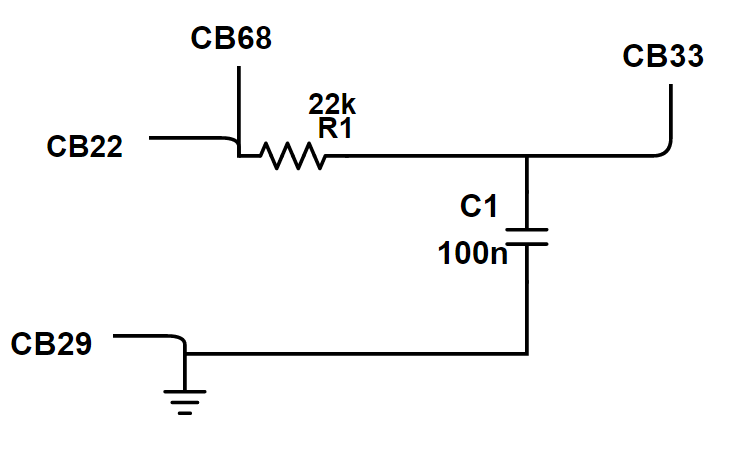
\includegraphics[width=0.7\linewidth]{./breadboard1_passabasso}
\caption{Circuito passa basso realizzato sulla breadboard.}
\label{fig:breadboard_1}
\end{figure}


Resistenza: $22 k\Omega \pm 5 $ \% tolleranza.
Condensatore: $68\si{nF}$, con permittività 10, di polipropilene.

Per questo circuito è prevista una frequenza di taglio di $f_T =\frac{1}{2\pi RC} = 106.4 \si{Hz}$.

All'interno del \textit{VI} è possibile impostare i valori iniziali per il range di acquisizione delle frequenze, il numero di misure (campionamento), il numero di periodi per ogni sinusoide e infine il fondoscala. I valori da noi usati per questa prima acquisizione sono:
\\

\begin{tabular}{|c|c|}
\hline range frequenze & 5-2000 \si{Hz} \\ 
\hline num. campionamenti & 30 \\ 
\hline num. periodi & 5 \\ 
\hline num. camp/periodo & 25 \\ 
\hline fondoscala & 5 \si{V} \\ 
\hline 
\end{tabular} \\


Ci aspettiamo che il comportamento del circuito sia quello di un filtro passa-basso (passivo), che tagli, cioè, le frequenze maggiori della frequenza di taglio, e lasci passare (attenuando poco) quelle minori di tale soglia. \\
I grafici ricostruiti da \textit{LabView} mostrano un andamento simile a quanto aspettato. In particolare viene chiesto quale potrebbe essere l'attenuazione (con tensione in ingresso normalizzata ad 1) per una frequenza di $10 \si{kH}$. Si può rispondere a questa domanda in più modi: partendo da un esame prettamente grafico notiamo che alla frequenza di circa $2000\si{kHz}$, l'attenuazione è circa $0.05$, in diminuzione per questo range di frequenze. Interpolando i punti sperimentali e prolungando la curva tracciata, risulta plausibile un valore dell'attenuazione dell'ordine di $10^{-2}$. \\
Alternativamente, possiamo analizzare il circuito scrivendo il modulo della funzione di trasferimento del circuito e la formula per lo sfasamento introdotto fra $V_{in}$ e $V_{out}$, che sono come segue:

\begin{equation}\label{F_trasf}
\rvert H(f) \lvert = \frac{1}{\sqrt{1+(\frac{f}{f_T})^2}}
\end{equation}

\begin{equation}
\Delta \phi = (-)\arctan(\frac{f}{f_T})
\end{equation}


E' interessante studiare il limitre asintotico per alte frequenze (alte rispetto alla frequenza di taglio), che ci fornisce un'ottima approssimazione del valore richiesto.

\begin{equation}
\rvert H(f) \lvert = \frac{1}{\sqrt{1+(\frac{f}{f_T})^2}}
\sim \frac{f_T}{f} 
= \frac{106.4 \si{Hz}}{10\si{kHz}} 
\approx 10 mV 
%(\mbox{per f \gg f_T})
\end{equation}


assolutamente compatibile con l'esame qualitativo precedente. Che il modello teorico risulti in accordo con i dati sperimentali (per $f \gg f_T$), lo si può vedere esaminando il grafico delle attenuazioni in scala bilog: se effettivamente l'andamento funzionale deve essere come $1/f$, ci aspettiamo che in scala bilog risulti una retta con pendenza circa $-1$, che è quanto risulta dal fit dei dati.

\begin{figure}
\centering
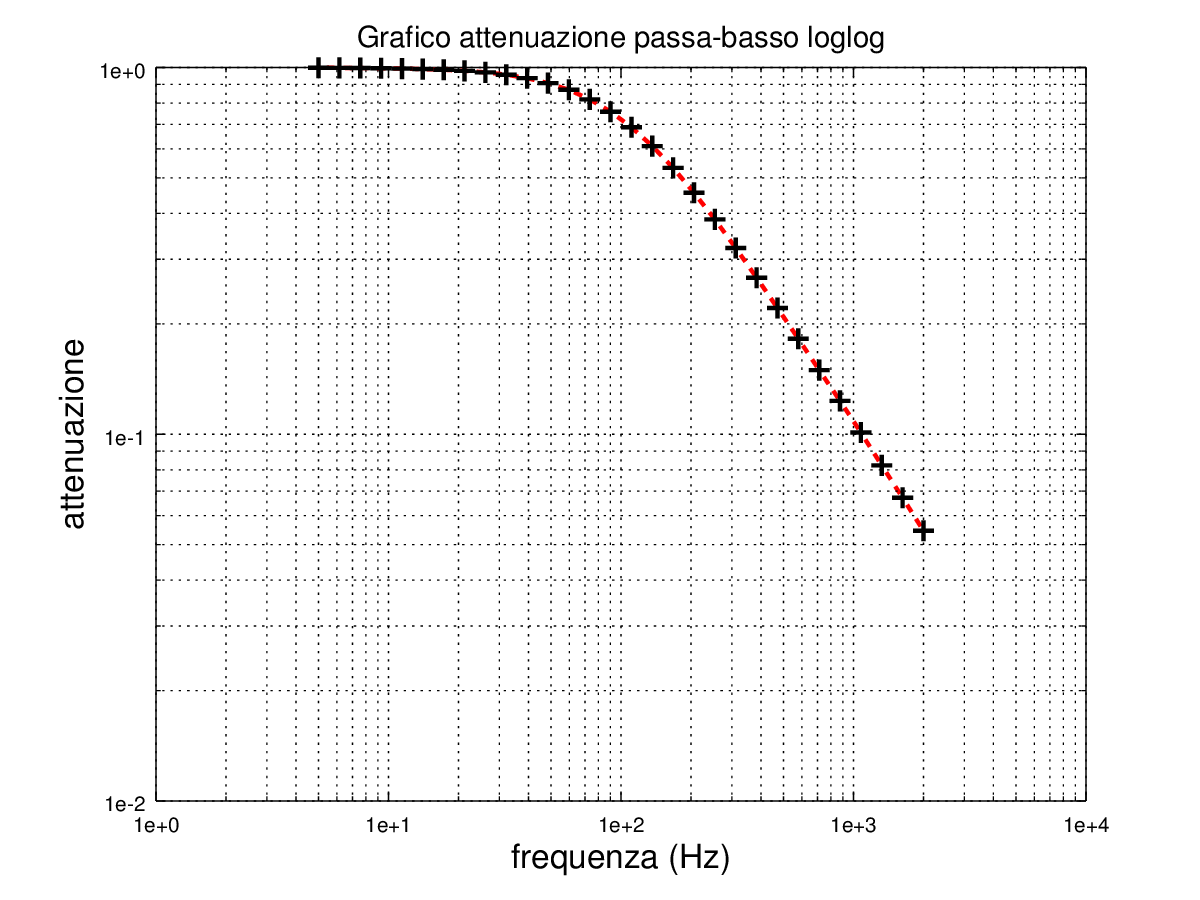
\includegraphics[width=1.1\linewidth]{./attenuaz_passa_basso_loglog}
\caption{Attenuazione in scala bilog del filtro passa-basso}
\label{fig:attenuaz_passa_basso_loglog}
\end{figure}



Cambiando i valori dei parametri di input nel \textit{VI} è stato osservato che la misura dello sfasamento diventa sempre meno accurata man mano che viene ridotto il numero di campionamenti per periodo. Una possibile spiegazione di questo fenomeno è che se i punti sperimentali sono pochi, diventa sempre più difficile per il calcolatore tracciare una forma d'onda precisa, di cui si possa calcolare lo sfasamento rispetto al segnale in ingresso.

Per le frequenze $f_{50} = 50 Hz$ e $f_{500} = 500 Hz$ i valori dell'attenuazione e dello sfasamento previsti dal modello sono riportati nella tabella seguente:\\

\begin{tabular}{|c|c|c|}
\hline  & $f_{50}$ & $f_{500}$ \\ 
\hline Attenuazione & $0.89$ & $0.19$ \\ 
\hline $\Delta \phi $& $(-)26$  & $(-)78$ \\ 
\hline 
\end{tabular} \\


\subsection{Analisi AC con TINA}
A questo punto, tramite il software \textsc{TINA}, è stato riprodotto il circuito da noi costruito sulla breadboard e sono state settate come frequenze per il generatore AC proprio  $f_{50}$ e $f_{500}$, per cui \textsc{TINA} ha gentilmente calcolato i valori dell'attenuazione e dello sfasamento per via simbolica. \\

\begin{tabular}{|c|c|c|}
\hline  & $f_{50}$ & $f_{500}$ \\ 
\hline $V_{in}$ & $1 \si{V}$ & $1 \si{V}$ \\ 
\hline $\Delta \phi $& $(-)25.17$  & $(-)77.99$ \\ 
\hline Tensione su C & $905 \si{mV}$ & $208.12 \si{mV}$ \\ 
\hline 
\end{tabular} \\

Cambiando la scala da logaritmica in lineare, il grafico restituito da \textsc{TINA} assume una forma a campana centrata sul primo valore della frequenza. In questa scala è possibile studiare meglio gli andamenti per basse frequenze che ci aspettiamo quadratico, e infatti sviluppando al primo termine non nullo in $x= f/f_T$, risulta in una parabola con la concavità rivolta verso il basso. \\
Gli andamenti per alte frequenze sono più chiaramente leggibili in scala logaritmica, in cui l'andamento lineare è palese.

Per la regione del grafico compresa fra $500-1000 \si{Hz}$ il guadagno di $-6db$ dimezzando la frequenza è perfettamente verificato. Altresì, tale guadagno viene mostrato alla frequenza di $180\si{Hz}$ e l'amplificazione del segnale è di $0.5$. Questa frequenza assume un'importanza particolare poichè, a partire dalla (\ref{F_trasf}), ponendo l'amplificazione pari a $1/2$ la $f_{1/2}$ alla quale questa si verifica è $f_{1/2}^{exp} = \sqrt{3}f_T = 184 \si{Hz} \approx f_{1/2} = 180 \si{Hz} $.\\

Come controprova sul circuito realizzato sperimentalmente, impostando una frequenza di start dello sweep $f_{start} = 160 \si{Hz}$ e una frequenza di end-sweep $f_{end} = 200 \si{Hz}$, otteniamo che in corrispondenza di un'amplificazione di $0.5$, si ha una frequenza pari circa a $f = 182.36 \si{Hz}$, in linea con quanto visto.

\subsection{Filtri passa-banda capacitivi}
Passiamo ora ad analizzare un filtro passa-banda capacitivo, composto da un filtro passa-basso collegato ad un filtro passa-alto. Riportiamo in Figura (\ref{fig:breadboard2_passabanda}) lo schema del circuito. \\

Sappiamo già che per avere un buon funzionamento della serie dei filtri è necessario che l'impedenza (vista dalla resistenza da $ 1 k\Omega $ ) del ramo contenente il condensatore da $ 100 nF $ deve essere molto minore di quella del ramo contenente il filto passa alto. Simbolicamente questo corrisponde a scrivere la condizione:

\begin{equation}
\frac{1}{j\omega C_2} + R_2 \gg \frac{1}{j\omega C_1}
\end{equation}

che nel nostro caso è ben verificata. Inoltre è necessario che le frequenze di lavoro siano molto minori di quella di taglio del passa basso e maggiori di quella del passa alto.

\begin{figure}
\centering
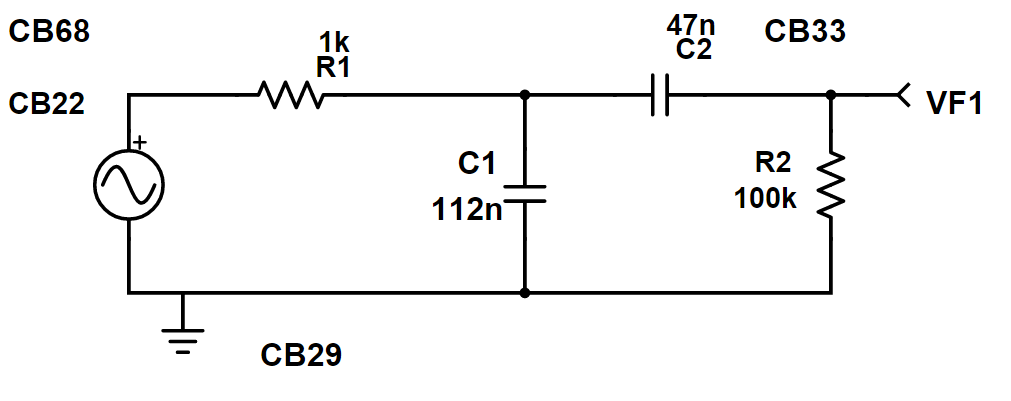
\includegraphics[width=0.7\linewidth]{./breadboard2_passabanda}
\caption{Schema del circuito passa-banda: date le capacità disponibili, C1 (inizialmente prevista di 100nF) è stata resa con un parallelo fra due capacità di 56nF ciascuna.}
\label{fig:breadboard2_passabanda}
\end{figure}


Le frequenze di taglio dei filtri sono:\\

\begin{tabular}{|c|c|}
\hline $f_{TA}$ & $f_{TB} $\\ 
\hline $1591 \si{Hz}$ & $33 \si{Hz}$ \\ 
\hline 
\end{tabular} \\

Poichè si tratta di una composizione di due filtri, lo sfasamento risulta essere la somma fra gli sfasamenti (uno è negativo e uno positivo), che in particolare risulta essere pari a zero per $f_0 = \sqrt{f_{T,A}f_{T,B}} $. Quindi, $f_0^{exp} = 232.11 \si{Hz}$, mentre quella interpolata graficamente dal diagramma \textsc{BODE} realizzato da \textsc{TINA}, è circa $230 \si{Hz}$. 

\begin{figure}
\centering
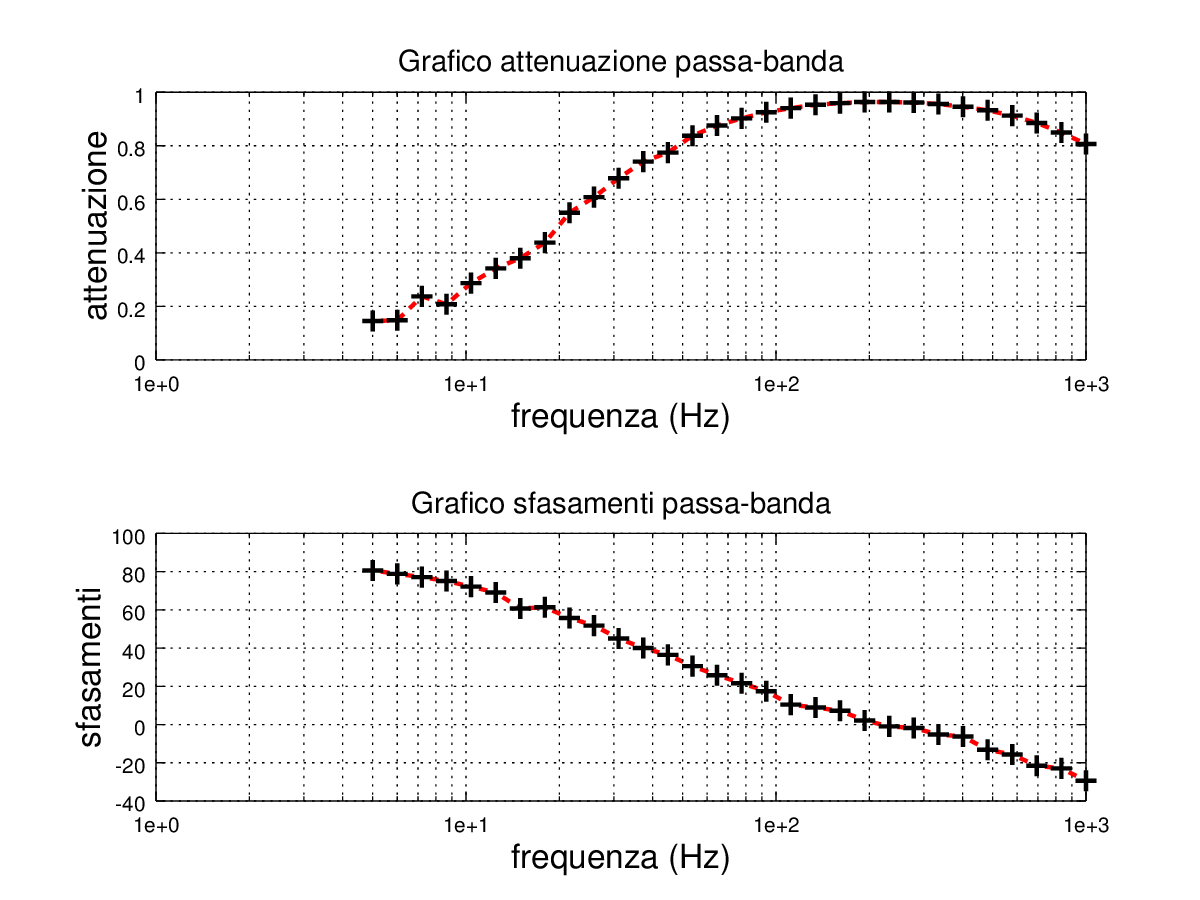
\includegraphics[width=1.1\linewidth]{./passabanda_sfasa_octave}
\caption{Grafico dell'attenuazione e dello sfasamento prodotto dal VI, acquisendo i dati dalla breadboard}
\label{fig:passabanda_sfasa_octave}
\end{figure}


Si può notare dalla figura (\ref{fig:passabanda_sfasa_octave}) acquisita con il \textit{VI}, che la regione in cui il guadagno è alto risulta piuttosto ampia, con frequenze appartenenti all'intervallo $80-800 \si{Hz}$. In altre parole, la larghezza del picco è grande. \\
Inoltre, per basse frequenze notiamo dei punti sperimentali sensibilmente scostati dalla spezzata prodotta dai restanti campionamenti. Per altre frequenze,invece, si evidenzia un buon accordo con l'andamento simulato con \textsc{Tina}. 

\section{Conclusion}
	This section summarizes the paper.

% Now we need a bibliography:
\begin{thebibliography}{5}

	%Each item starts with a \bibitem{reference} command and the details thereafter.
	\bibitem{HOP96} % Transaction paper
	J.~Hagenauer, E.~Offer, and L.~Papke. Iterative decoding of binary block
	and convolutional codes. {\em IEEE Trans. Inform. Theory},
	vol.~42, no.~2, pp.~429–-445, Mar. 1996.

	\bibitem{MJH06} % Conference paper
	T.~Mayer, H.~Jenkac, and J.~Hagenauer. Turbo base-station cooperation for intercell interference cancellation. {\em IEEE Int. Conf. Commun. (ICC)}, Istanbul, Turkey, pp.~356--361, June 2006.

	\bibitem{Proakis} % Book
	J.~G.~Proakis. {\em Digital Communications}. McGraw-Hill Book Co.,
	New York, USA, 3rd edition, 1995.

	\bibitem{talk} % Web document
	F.~R.~Kschischang. Giving a talk: Guidelines for the Preparation and Presentation of Technical Seminars.
	\url{http://www.comm.toronto.edu/frank/guide/guide.pdf}.

	\bibitem{5}
	IEEE Transactions \LaTeX and Microsoft Word Style Files.
	\url{http://www.ieee.org/web/publications/authors/transjnl/index.html}

\end{thebibliography}

% Your document ends here!
\end{document}
